% Options for packages loaded elsewhere
\PassOptionsToPackage{unicode}{hyperref}
\PassOptionsToPackage{hyphens}{url}
\PassOptionsToPackage{dvipsnames,svgnames,x11names}{xcolor}
%
\documentclass[
  11pt,
  a4paper,
]{article}

\usepackage{amsmath,amssymb}
\usepackage{setspace}
\usepackage{iftex}
\ifPDFTeX
  \usepackage[T1]{fontenc}
  \usepackage[utf8]{inputenc}
  \usepackage{textcomp} % provide euro and other symbols
\else % if luatex or xetex
  \usepackage{unicode-math}
  \defaultfontfeatures{Scale=MatchLowercase}
  \defaultfontfeatures[\rmfamily]{Ligatures=TeX,Scale=1}
\fi
\usepackage{lmodern}
\ifPDFTeX\else  
    % xetex/luatex font selection
    \setmainfont[]{Times New Roman}
    \setsansfont[]{Arial}
    \setmonofont[]{Courier New}
\fi
% Use upquote if available, for straight quotes in verbatim environments
\IfFileExists{upquote.sty}{\usepackage{upquote}}{}
\IfFileExists{microtype.sty}{% use microtype if available
  \usepackage[]{microtype}
  \UseMicrotypeSet[protrusion]{basicmath} % disable protrusion for tt fonts
}{}
\makeatletter
\@ifundefined{KOMAClassName}{% if non-KOMA class
  \IfFileExists{parskip.sty}{%
    \usepackage{parskip}
  }{% else
    \setlength{\parindent}{0pt}
    \setlength{\parskip}{6pt plus 2pt minus 1pt}}
}{% if KOMA class
  \KOMAoptions{parskip=half}}
\makeatother
\usepackage{xcolor}
\usepackage[margin=2.5cm]{geometry}
\setlength{\emergencystretch}{3em} % prevent overfull lines
\setcounter{secnumdepth}{3}
% Make \paragraph and \subparagraph free-standing
\makeatletter
\ifx\paragraph\undefined\else
  \let\oldparagraph\paragraph
  \renewcommand{\paragraph}{
    \@ifstar
      \xxxParagraphStar
      \xxxParagraphNoStar
  }
  \newcommand{\xxxParagraphStar}[1]{\oldparagraph*{#1}\mbox{}}
  \newcommand{\xxxParagraphNoStar}[1]{\oldparagraph{#1}\mbox{}}
\fi
\ifx\subparagraph\undefined\else
  \let\oldsubparagraph\subparagraph
  \renewcommand{\subparagraph}{
    \@ifstar
      \xxxSubParagraphStar
      \xxxSubParagraphNoStar
  }
  \newcommand{\xxxSubParagraphStar}[1]{\oldsubparagraph*{#1}\mbox{}}
  \newcommand{\xxxSubParagraphNoStar}[1]{\oldsubparagraph{#1}\mbox{}}
\fi
\makeatother

\usepackage{color}
\usepackage{fancyvrb}
\newcommand{\VerbBar}{|}
\newcommand{\VERB}{\Verb[commandchars=\\\{\}]}
\DefineVerbatimEnvironment{Highlighting}{Verbatim}{commandchars=\\\{\}}
% Add ',fontsize=\small' for more characters per line
\usepackage{framed}
\definecolor{shadecolor}{RGB}{241,243,245}
\newenvironment{Shaded}{\begin{snugshade}}{\end{snugshade}}
\newcommand{\AlertTok}[1]{\textcolor[rgb]{0.68,0.00,0.00}{#1}}
\newcommand{\AnnotationTok}[1]{\textcolor[rgb]{0.37,0.37,0.37}{#1}}
\newcommand{\AttributeTok}[1]{\textcolor[rgb]{0.40,0.45,0.13}{#1}}
\newcommand{\BaseNTok}[1]{\textcolor[rgb]{0.68,0.00,0.00}{#1}}
\newcommand{\BuiltInTok}[1]{\textcolor[rgb]{0.00,0.23,0.31}{#1}}
\newcommand{\CharTok}[1]{\textcolor[rgb]{0.13,0.47,0.30}{#1}}
\newcommand{\CommentTok}[1]{\textcolor[rgb]{0.37,0.37,0.37}{#1}}
\newcommand{\CommentVarTok}[1]{\textcolor[rgb]{0.37,0.37,0.37}{\textit{#1}}}
\newcommand{\ConstantTok}[1]{\textcolor[rgb]{0.56,0.35,0.01}{#1}}
\newcommand{\ControlFlowTok}[1]{\textcolor[rgb]{0.00,0.23,0.31}{\textbf{#1}}}
\newcommand{\DataTypeTok}[1]{\textcolor[rgb]{0.68,0.00,0.00}{#1}}
\newcommand{\DecValTok}[1]{\textcolor[rgb]{0.68,0.00,0.00}{#1}}
\newcommand{\DocumentationTok}[1]{\textcolor[rgb]{0.37,0.37,0.37}{\textit{#1}}}
\newcommand{\ErrorTok}[1]{\textcolor[rgb]{0.68,0.00,0.00}{#1}}
\newcommand{\ExtensionTok}[1]{\textcolor[rgb]{0.00,0.23,0.31}{#1}}
\newcommand{\FloatTok}[1]{\textcolor[rgb]{0.68,0.00,0.00}{#1}}
\newcommand{\FunctionTok}[1]{\textcolor[rgb]{0.28,0.35,0.67}{#1}}
\newcommand{\ImportTok}[1]{\textcolor[rgb]{0.00,0.46,0.62}{#1}}
\newcommand{\InformationTok}[1]{\textcolor[rgb]{0.37,0.37,0.37}{#1}}
\newcommand{\KeywordTok}[1]{\textcolor[rgb]{0.00,0.23,0.31}{\textbf{#1}}}
\newcommand{\NormalTok}[1]{\textcolor[rgb]{0.00,0.23,0.31}{#1}}
\newcommand{\OperatorTok}[1]{\textcolor[rgb]{0.37,0.37,0.37}{#1}}
\newcommand{\OtherTok}[1]{\textcolor[rgb]{0.00,0.23,0.31}{#1}}
\newcommand{\PreprocessorTok}[1]{\textcolor[rgb]{0.68,0.00,0.00}{#1}}
\newcommand{\RegionMarkerTok}[1]{\textcolor[rgb]{0.00,0.23,0.31}{#1}}
\newcommand{\SpecialCharTok}[1]{\textcolor[rgb]{0.37,0.37,0.37}{#1}}
\newcommand{\SpecialStringTok}[1]{\textcolor[rgb]{0.13,0.47,0.30}{#1}}
\newcommand{\StringTok}[1]{\textcolor[rgb]{0.13,0.47,0.30}{#1}}
\newcommand{\VariableTok}[1]{\textcolor[rgb]{0.07,0.07,0.07}{#1}}
\newcommand{\VerbatimStringTok}[1]{\textcolor[rgb]{0.13,0.47,0.30}{#1}}
\newcommand{\WarningTok}[1]{\textcolor[rgb]{0.37,0.37,0.37}{\textit{#1}}}

\providecommand{\tightlist}{%
  \setlength{\itemsep}{0pt}\setlength{\parskip}{0pt}}\usepackage{longtable,booktabs,array}
\usepackage{calc} % for calculating minipage widths
% Correct order of tables after \paragraph or \subparagraph
\usepackage{etoolbox}
\makeatletter
\patchcmd\longtable{\par}{\if@noskipsec\mbox{}\fi\par}{}{}
\makeatother
% Allow footnotes in longtable head/foot
\IfFileExists{footnotehyper.sty}{\usepackage{footnotehyper}}{\usepackage{footnote}}
\makesavenoteenv{longtable}
\usepackage{graphicx}
\makeatletter
\newsavebox\pandoc@box
\newcommand*\pandocbounded[1]{% scales image to fit in text height/width
  \sbox\pandoc@box{#1}%
  \Gscale@div\@tempa{\textheight}{\dimexpr\ht\pandoc@box+\dp\pandoc@box\relax}%
  \Gscale@div\@tempb{\linewidth}{\wd\pandoc@box}%
  \ifdim\@tempb\p@<\@tempa\p@\let\@tempa\@tempb\fi% select the smaller of both
  \ifdim\@tempa\p@<\p@\scalebox{\@tempa}{\usebox\pandoc@box}%
  \else\usebox{\pandoc@box}%
  \fi%
}
% Set default figure placement to htbp
\def\fps@figure{htbp}
\makeatother

\usepackage{fvextra}
\DefineVerbatimEnvironment{Highlighting}{Verbatim}{breaklines=true,breakanywhere=true,commandchars=\\\{\}}
\RecustomVerbatimEnvironment{Verbatim}{Verbatim}{breaklines=true,breakanywhere=true,frame=single}
\makeatletter
\@ifpackageloaded{caption}{}{\usepackage{caption}}
\AtBeginDocument{%
\ifdefined\contentsname
  \renewcommand*\contentsname{Table of contents}
\else
  \newcommand\contentsname{Table of contents}
\fi
\ifdefined\listfigurename
  \renewcommand*\listfigurename{List of Figures}
\else
  \newcommand\listfigurename{List of Figures}
\fi
\ifdefined\listtablename
  \renewcommand*\listtablename{List of Tables}
\else
  \newcommand\listtablename{List of Tables}
\fi
\ifdefined\figurename
  \renewcommand*\figurename{Figure}
\else
  \newcommand\figurename{Figure}
\fi
\ifdefined\tablename
  \renewcommand*\tablename{Table}
\else
  \newcommand\tablename{Table}
\fi
}
\@ifpackageloaded{float}{}{\usepackage{float}}
\floatstyle{ruled}
\@ifundefined{c@chapter}{\newfloat{codelisting}{h}{lop}}{\newfloat{codelisting}{h}{lop}[chapter]}
\floatname{codelisting}{Listing}
\newcommand*\listoflistings{\listof{codelisting}{List of Listings}}
\makeatother
\makeatletter
\makeatother
\makeatletter
\@ifpackageloaded{caption}{}{\usepackage{caption}}
\@ifpackageloaded{subcaption}{}{\usepackage{subcaption}}
\makeatother
\makeatletter
\@ifpackageloaded{tcolorbox}{}{\usepackage[skins,breakable]{tcolorbox}}
\makeatother
\makeatletter
\@ifundefined{shadecolor}{\definecolor{shadecolor}{rgb}{.97, .97, .97}}{}
\makeatother
\makeatletter
\makeatother
\makeatletter
\ifdefined\Shaded\renewenvironment{Shaded}{\begin{tcolorbox}[enhanced, borderline west={3pt}{0pt}{shadecolor}, interior hidden, sharp corners, boxrule=0pt, breakable, frame hidden]}{\end{tcolorbox}}\fi
\makeatother

\usepackage{bookmark}

\IfFileExists{xurl.sty}{\usepackage{xurl}}{} % add URL line breaks if available
\urlstyle{same} % disable monospaced font for URLs
\hypersetup{
  pdftitle={Redes bayesianas gaussianas},
  pdfauthor={Oliver Arturo Casas Pontanillo \textbar{} A01645764; Erik Abraham Jajan Díaz \textbar{} A01644648; José Luis Santos Montaño \textbar{} A01781721},
  colorlinks=true,
  linkcolor={blue},
  filecolor={Maroon},
  citecolor={Blue},
  urlcolor={Blue},
  pdfcreator={LaTeX via pandoc}}


\title{Redes bayesianas gaussianas}
\author{Oliver Arturo Casas Pontanillo \textbar{} A01645764 \and Erik
Abraham Jajan Díaz \textbar{} A01644648 \and José Luis Santos Montaño
\textbar{} A01781721}
\date{2025-09-07}

\begin{document}
\maketitle

\renewcommand*\contentsname{Table of contents}
{
\hypersetup{linkcolor=}
\setcounter{tocdepth}{3}
\tableofcontents
}

\setstretch{1.5}
https://github.com/olivercasas17/MA2014\_Redes\_bayesianas\_gaussianas

\subsection{Abstract}\label{abstract}

Esta investigación examina las relaciones entre contaminantes
atmosféricos y biomarcadores de salud mediante redes bayesianas
gaussianas. Utilizando datos de ENSANUT 2022 y calidad del aire de
SEMARNAT, se modelaron las dependencias entre siete contaminantes y diez
biomarcadores sanguíneos. Se construyeron tres DAGs alternativos y se
seleccionó el modelo óptimo mediante criterios AIC y BIC. Los resultados
proporcionan evidencia cuantitativa del impacto de la contaminación
atmosférica en biomarcadores metabólicos, lipídicos e inflamatorios,
contribuyendo al diseño de políticas de salud ambiental.

\subsection{Introducción}\label{introducciuxf3n}

Diversos estudios han demostrado que la exposición crónica a
contaminantes atmosféricos se asocia con un aumento en enfermedades
respiratorias, cardiovasculares y metabólicas. Estos efectos usualmente
se manifiestan en biomarcadores biológicos, los cuales permiten que se
evalúe de manera indirecta el impacto de los contaminantes en la salud
de las personas.~ Las redes bayesianas gaussianas nos permiten modelar
las dependencias probabilísticas entre variables y generar
representaciones gráficas. En este caso, el uso de los datos
provenientes de la encuesta nacional ENSANUT 2022, que ofrecen
información detallada sobre muestras de sangre e información
sociodemográfica, además de información actualizada de la SEMARNAT sobre
los contaminantes del aire, nos permitirán \emph{plantear como hipótesis
que los contaminantes atmosféricos tienen un efecto significativo sobre
determinados biomarcadores de salud.} ~ Comprender cómo interactúan
factores ambientales con los biomarcadores de salud de la población
genera un impacto importante, ya que puede contribuir al diseño de
políticas públicas orientadas a la prevención y mitigación de los
efectos de la contaminación atmosférica.

\subsection{Metodología}\label{metodologuxeda}

El trabajo sigue un enfoque cuantitativo, exploratorio, explicativo e
interdisciplinario, analizando las relaciones que tienen contaminantes
del aire con biomarcadores de salud en la población, utilizando redes
bayesianas gaussianas para representar estas relaciones de variables
continuas.~ Inicialmente, se realizó una limpieza de la base de datos
para extraer las variables con datos continuos relevantes para nuestro
estudio, además de asegurarnos de que los datos estuvieran en un formato
con el que pudiéramos trabajar.~ Basándonos en información proporcionada
por especialistas, se propusieron tres gráficos acíclicos dirigidos, por
sus siglas en inglés DAGs, para posteriormente comparar las 3 DAGs con
métricas estadísticas, y seleccionar la mejor de las tres para continuar
con el análisis. ~ Se incluyó una variable categórica específica, en
este caso sexo, y con ayuda de los especialistas en el tema se
escogieron tres queries que nos llevarían a conclusiones prometedoras~
Las principales técnicas que se utilizaron en este trabajo fueron: ~
Análisis de redes bayesianas gaussianas, construyendo grafos acíclicos
dirigidos para modelar relaciones de dependencia entre variables
continuas~ Evaluación de modelos, usando métodos estadísticos como el
Criterio de Información de Akaike y el Criterio de Información
Bayesiano, AIC y BIC por sus siglas en inglés.~ Inferencia
probabilística, consultas condicionales para estimar probabilidades bajo
evidencia~ Los datos utilizados fueron los siguientes:~ data.csv~
data\_F.csv~ data\_M.csv~ Los datos crudos fueron recolectados de:~
calidad\_aire\_2025.csv~ ensanut2022\_muestras.csv~
ensanut2022\_socdem.csv~ Las herramientas que utilizamos fueron las
siguientes:~ Lenguaje de programación R~ Librerías: tidyverse, bnlearn,
Rgraphviz~ Entorno de trabajo R Studio

\subsection{Aplicacion}\label{aplicacion}

\begin{Shaded}
\begin{Highlighting}[numbers=left,,]
\FunctionTok{library}\NormalTok{(tidyverse)}
\FunctionTok{library}\NormalTok{(bnlearn)}
\end{Highlighting}
\end{Shaded}

\begin{Shaded}
\begin{Highlighting}[numbers=left,,]
\NormalTok{data }\OtherTok{=} \FunctionTok{read\_csv}\NormalTok{(}\StringTok{"../data/data.csv"}\NormalTok{)}
\FunctionTok{head}\NormalTok{(data)}
\end{Highlighting}
\end{Shaded}

\begin{verbatim}
# A tibble: 6 x 17
  valor_ALBU valor_COL_HDL valor_COL_LDL valor_CREAT valor_GLU_SUERO
       <dbl>         <dbl>         <dbl>       <dbl>           <dbl>
1        3.8            73           130        0.62             111
2        4.1            49           107        0.91             106
3        4.2            41            76        0.71             109
4        3.8            42            84        0.65              98
5        4.1            41           119        0.83             253
6        3.8            44           133        0.66             204
# i 12 more variables: valor_INSULINA <dbl>, valor_PCR <dbl>, valor_TRIG <dbl>,
#   valor_EAG <dbl>, valor_HB1AC <dbl>, SO_2 <dbl>, CO <dbl>, NOx <dbl>,
#   COV <dbl>, PM_010 <dbl>, PM_2_5 <dbl>, NH_3 <dbl>
\end{verbatim}

\begin{Shaded}
\begin{Highlighting}[numbers=left,,]
\FunctionTok{colnames}\NormalTok{(data) }\OtherTok{\textless{}{-}} \FunctionTok{c}\NormalTok{(}\StringTok{"ALB"}\NormalTok{, }\StringTok{"HDL"}\NormalTok{, }\StringTok{"LDL"}\NormalTok{, }\StringTok{"CR"}\NormalTok{, }\StringTok{"GLU"}\NormalTok{, }\StringTok{"INS"}\NormalTok{, }\StringTok{"PCR"}\NormalTok{, }\StringTok{"TRI"}\NormalTok{, }\StringTok{"HB1AC"}\NormalTok{, }\StringTok{"EAG"}\NormalTok{, }\StringTok{"SO2"}\NormalTok{, }\StringTok{"CO"}\NormalTok{, }\StringTok{"NOx"}\NormalTok{, }\StringTok{"COV"}\NormalTok{, }\StringTok{"PM10"}\NormalTok{, }\StringTok{"PM2.5"}\NormalTok{, }\StringTok{"NH3"}\NormalTok{)}
\end{Highlighting}
\end{Shaded}

\begin{Shaded}
\begin{Highlighting}[numbers=left,,]
\NormalTok{dag1 }\OtherTok{=} \FunctionTok{empty.graph}\NormalTok{(}\AttributeTok{nodes =} \FunctionTok{c}\NormalTok{(}\StringTok{"ALB"}\NormalTok{, }\StringTok{"HDL"}\NormalTok{, }\StringTok{"LDL"}\NormalTok{, }\StringTok{"CR"}\NormalTok{, }\StringTok{"GLU"}\NormalTok{, }\StringTok{"INS"}\NormalTok{, }\StringTok{"PCR"}\NormalTok{, }\StringTok{"TRI"}\NormalTok{, }\StringTok{"HB1AC"}\NormalTok{, }\StringTok{"EAG"}\NormalTok{, }\StringTok{"SO2"}\NormalTok{, }\StringTok{"CO"}\NormalTok{, }\StringTok{"NOx"}\NormalTok{, }\StringTok{"COV"}\NormalTok{, }\StringTok{"PM10"}\NormalTok{, }\StringTok{"PM2.5"}\NormalTok{, }\StringTok{"NH3"}\NormalTok{))}
\end{Highlighting}
\end{Shaded}

\begin{Shaded}
\begin{Highlighting}[numbers=left,,]
\NormalTok{arc\_set1 }\OtherTok{=} \FunctionTok{matrix}\NormalTok{(}\FunctionTok{c}\NormalTok{(}\StringTok{"TRI"}\NormalTok{, }\StringTok{"LDL"}\NormalTok{,}
                   \StringTok{"TRI"}\NormalTok{, }\StringTok{"HDL"}\NormalTok{,}
                   \StringTok{"INS"}\NormalTok{, }\StringTok{"LDL"}\NormalTok{,}
                   \StringTok{"INS"}\NormalTok{, }\StringTok{"HDL"}\NormalTok{,}
                   \StringTok{"GLU"}\NormalTok{, }\StringTok{"INS"}\NormalTok{,}
                   \StringTok{"GLU"}\NormalTok{, }\StringTok{"HB1AC"}\NormalTok{,}
                   \StringTok{"GLU"}\NormalTok{, }\StringTok{"PCR"}\NormalTok{,}
                   \StringTok{"GLU"}\NormalTok{, }\StringTok{"CR"}\NormalTok{,}
                   \StringTok{"INS"}\NormalTok{, }\StringTok{"CR"}\NormalTok{,}
                   \StringTok{"INS"}\NormalTok{, }\StringTok{"PCR"}\NormalTok{,}
                   \StringTok{"HB1AC"}\NormalTok{, }\StringTok{"EAG"}\NormalTok{,}
                   \StringTok{"HB1AC"}\NormalTok{, }\StringTok{"PCR"}\NormalTok{,}
                   \StringTok{"EAG"}\NormalTok{, }\StringTok{"PCR"}\NormalTok{,}
                   \StringTok{"CR"}\NormalTok{, }\StringTok{"ALB"}\NormalTok{,}
                   \StringTok{"SO2"}\NormalTok{, }\StringTok{"ALB"}\NormalTok{,}
                   \StringTok{"SO2"}\NormalTok{, }\StringTok{"PCR"}\NormalTok{,}
                   \StringTok{"CO"}\NormalTok{, }\StringTok{"CR"}\NormalTok{,}
                   \StringTok{"CO"}\NormalTok{, }\StringTok{"HB1AC"}\NormalTok{,}
                   \StringTok{"NOx"}\NormalTok{, }\StringTok{"TRI"}\NormalTok{,}
                   \StringTok{"COV"}\NormalTok{, }\StringTok{"GLU"}\NormalTok{,}
                   \StringTok{"PM10"}\NormalTok{, }\StringTok{"PCR"}\NormalTok{,}
                   \StringTok{"PM2.5"}\NormalTok{, }\StringTok{"GLU"}\NormalTok{,}
                   \StringTok{"NH3"}\NormalTok{, }\StringTok{"PCR"}\NormalTok{,}
                   \StringTok{"NH3"}\NormalTok{, }\StringTok{"ALB"}\NormalTok{), }\AttributeTok{byrow =} \ConstantTok{TRUE}\NormalTok{, }\AttributeTok{ncol =} \DecValTok{2}\NormalTok{,}
                 \AttributeTok{dimnames =} \FunctionTok{list}\NormalTok{(}\ConstantTok{NULL}\NormalTok{, }\FunctionTok{c}\NormalTok{(}\StringTok{"from"}\NormalTok{, }\StringTok{"to"}\NormalTok{)))}
\end{Highlighting}
\end{Shaded}

\begin{Shaded}
\begin{Highlighting}[numbers=left,,]
\FunctionTok{arcs}\NormalTok{(dag1) }\OtherTok{=}\NormalTok{ arc\_set1}
\end{Highlighting}
\end{Shaded}

\begin{Shaded}
\begin{Highlighting}[numbers=left,,]
\FunctionTok{graphviz.plot}\NormalTok{(dag1, }\AttributeTok{shape =} \StringTok{"ellipse"}\NormalTok{)}
\end{Highlighting}
\end{Shaded}

\begin{verbatim}
Loading required namespace: Rgraphviz
\end{verbatim}

\pandocbounded{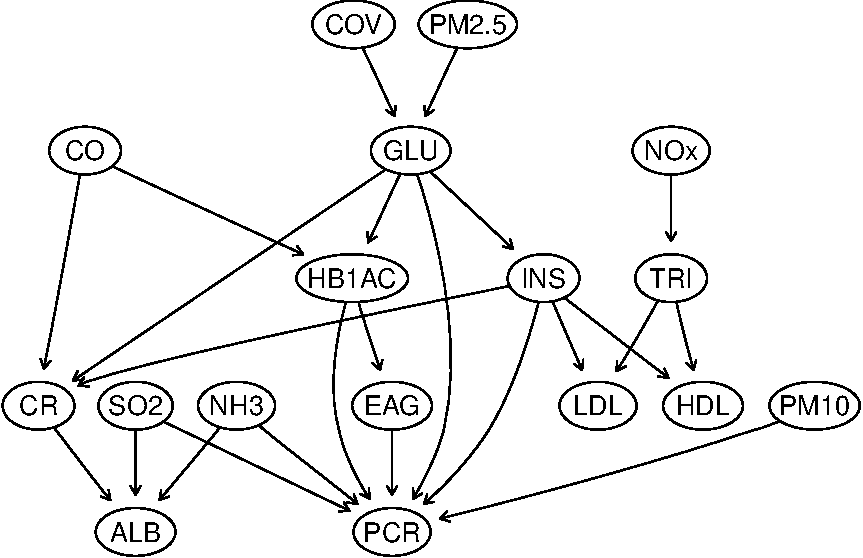
\includegraphics[keepaspectratio]{Reporte_files/figure-pdf/unnamed-chunk-7-1.pdf}}

\begin{Shaded}
\begin{Highlighting}[numbers=left,,]
\NormalTok{gbn1 }\OtherTok{=} \FunctionTok{bn.fit}\NormalTok{(dag1, }\AttributeTok{data =}\NormalTok{ data)}
\end{Highlighting}
\end{Shaded}

\begin{Shaded}
\begin{Highlighting}[numbers=left,,]
\NormalTok{score\_bic\_dag1 }\OtherTok{=} \FunctionTok{score}\NormalTok{(dag1, }\AttributeTok{data =}\NormalTok{ data, }\AttributeTok{type =} \StringTok{"bic{-}g"}\NormalTok{)}
\NormalTok{score\_bic\_dag1}
\end{Highlighting}
\end{Shaded}

\begin{verbatim}
[1] -97442.1
\end{verbatim}

\begin{Shaded}
\begin{Highlighting}[numbers=left,,]
\NormalTok{score\_aic\_dag1 }\OtherTok{=} \FunctionTok{score}\NormalTok{(dag1, }\AttributeTok{data =}\NormalTok{ data, }\AttributeTok{type =} \StringTok{"aic{-}g"}\NormalTok{)}
\NormalTok{score\_aic\_dag1}
\end{Highlighting}
\end{Shaded}

\begin{verbatim}
[1] -97297.73
\end{verbatim}

DAG 2:

\begin{Shaded}
\begin{Highlighting}[numbers=left,,]
\NormalTok{dag2 }\OtherTok{=} \FunctionTok{empty.graph}\NormalTok{(}\AttributeTok{nodes =} \FunctionTok{c}\NormalTok{(}\StringTok{"ALB"}\NormalTok{, }\StringTok{"HDL"}\NormalTok{, }\StringTok{"LDL"}\NormalTok{, }\StringTok{"TRI"}\NormalTok{, }\StringTok{"GLU"}\NormalTok{, }\StringTok{"INS"}\NormalTok{, }\StringTok{"PCR"}\NormalTok{, }
                              \StringTok{"HB1AC"}\NormalTok{, }\StringTok{"EAG"}\NormalTok{, }\StringTok{"CR"}\NormalTok{, }
                              \StringTok{"SO2"}\NormalTok{, }\StringTok{"CO"}\NormalTok{, }\StringTok{"NOx"}\NormalTok{, }\StringTok{"COV"}\NormalTok{, }\StringTok{"PM10"}\NormalTok{, }\StringTok{"PM2.5"}\NormalTok{, }\StringTok{"NH3"}\NormalTok{))}
\end{Highlighting}
\end{Shaded}

\begin{Shaded}
\begin{Highlighting}[numbers=left,,]
\NormalTok{arc\_set2 }\OtherTok{=} \FunctionTok{matrix}\NormalTok{(}\FunctionTok{c}\NormalTok{(}\StringTok{"SO2"}\NormalTok{, }\StringTok{"PCR"}\NormalTok{,}
                    \StringTok{"NOx"}\NormalTok{, }\StringTok{"PCR"}\NormalTok{,}
                    \StringTok{"COV"}\NormalTok{, }\StringTok{"PCR"}\NormalTok{,}
                    \StringTok{"PM10"}\NormalTok{, }\StringTok{"PCR"}\NormalTok{,}
                    \StringTok{"PM2.5"}\NormalTok{, }\StringTok{"PCR"}\NormalTok{,}
                    \StringTok{"CO"}\NormalTok{, }\StringTok{"PCR"}\NormalTok{,}
                    \StringTok{"NH3"}\NormalTok{, }\StringTok{"PCR"}\NormalTok{,}
                    \StringTok{"PCR"}\NormalTok{, }\StringTok{"ALB"}\NormalTok{,}
                    \StringTok{"NH3"}\NormalTok{, }\StringTok{"CR"}\NormalTok{,}
                    \StringTok{"CO"}\NormalTok{, }\StringTok{"CR"}\NormalTok{,}
                    \StringTok{"GLU"}\NormalTok{, }\StringTok{"INS"}\NormalTok{,}
                    \StringTok{"GLU"}\NormalTok{, }\StringTok{"HB1AC"}\NormalTok{,}
                    \StringTok{"HB1AC"}\NormalTok{, }\StringTok{"EAG"}\NormalTok{,}
                    \StringTok{"INS"}\NormalTok{, }\StringTok{"HDL"}\NormalTok{,}
                    \StringTok{"INS"}\NormalTok{, }\StringTok{"LDL"}\NormalTok{,}
                    \StringTok{"INS"}\NormalTok{, }\StringTok{"TRI"}\NormalTok{,}
                    \StringTok{"PCR"}\NormalTok{, }\StringTok{"GLU"}\NormalTok{), }\AttributeTok{byrow =} \ConstantTok{TRUE}\NormalTok{, }\AttributeTok{ncol =} \DecValTok{2}\NormalTok{,}
                  \AttributeTok{dimnames =} \FunctionTok{list}\NormalTok{(}\ConstantTok{NULL}\NormalTok{, }\FunctionTok{c}\NormalTok{(}\StringTok{"from"}\NormalTok{, }\StringTok{"to"}\NormalTok{)))}
\end{Highlighting}
\end{Shaded}

\begin{Shaded}
\begin{Highlighting}[numbers=left,,]
\FunctionTok{arcs}\NormalTok{(dag2) }\OtherTok{=}\NormalTok{ arc\_set2}
\end{Highlighting}
\end{Shaded}

\begin{Shaded}
\begin{Highlighting}[numbers=left,,]
\FunctionTok{graphviz.plot}\NormalTok{(dag2, }\AttributeTok{shape =} \StringTok{"ellipse"}\NormalTok{)}
\end{Highlighting}
\end{Shaded}

\pandocbounded{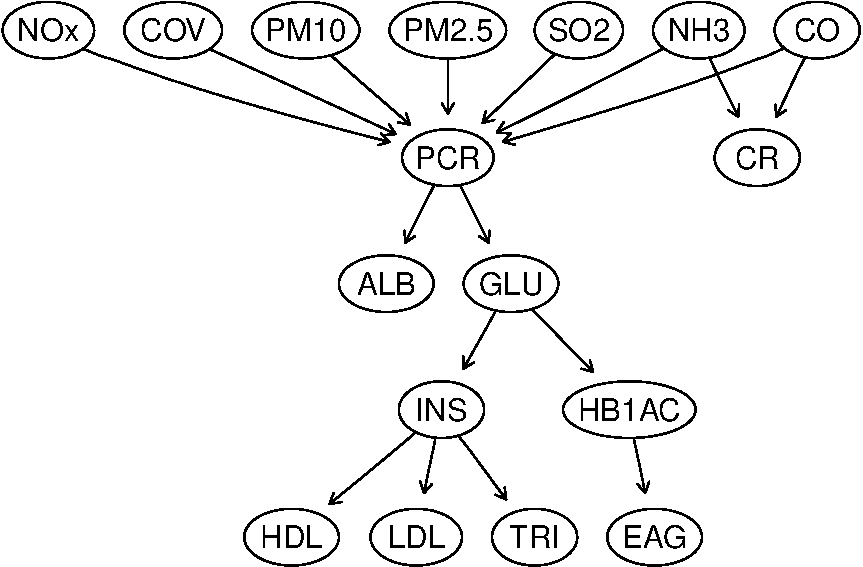
\includegraphics[keepaspectratio]{Reporte_files/figure-pdf/unnamed-chunk-14-1.pdf}}

\begin{Shaded}
\begin{Highlighting}[numbers=left,,]
\NormalTok{gbn2 }\OtherTok{=} \FunctionTok{bn.fit}\NormalTok{(dag2, }\AttributeTok{data =}\NormalTok{ data)}
\end{Highlighting}
\end{Shaded}

\begin{Shaded}
\begin{Highlighting}[numbers=left,,]
\NormalTok{score\_bic\_dag2 }\OtherTok{=} \FunctionTok{score}\NormalTok{(dag2, }\AttributeTok{data =}\NormalTok{ data, }\AttributeTok{type =} \StringTok{"bic{-}g"}\NormalTok{)}
\NormalTok{score\_bic\_dag2}
\end{Highlighting}
\end{Shaded}

\begin{verbatim}
[1] -97471.69
\end{verbatim}

\begin{Shaded}
\begin{Highlighting}[numbers=left,,]
\NormalTok{score\_aic\_dag2 }\OtherTok{=} \FunctionTok{score}\NormalTok{(dag2, }\AttributeTok{data =}\NormalTok{ data, }\AttributeTok{type =} \StringTok{"aic{-}g"}\NormalTok{)}
\NormalTok{score\_aic\_dag2}
\end{Highlighting}
\end{Shaded}

\begin{verbatim}
[1] -97344.75
\end{verbatim}

DAG 3:

\begin{Shaded}
\begin{Highlighting}[numbers=left,,]
\NormalTok{dag3 }\OtherTok{=} \FunctionTok{empty.graph}\NormalTok{(}\AttributeTok{nodes =} \FunctionTok{c}\NormalTok{(}\StringTok{"ALB"}\NormalTok{, }\StringTok{"HDL"}\NormalTok{, }\StringTok{"LDL"}\NormalTok{, }\StringTok{"CR"}\NormalTok{, }\StringTok{"GLU"}\NormalTok{,                                  }\StringTok{"INS"}\NormalTok{, }\StringTok{"PCR"}\NormalTok{, }\StringTok{"TRI"}\NormalTok{, }\StringTok{"HB1AC"}\NormalTok{, }
                             \StringTok{"EAG"}\NormalTok{, }\StringTok{"SO2"}\NormalTok{, }\StringTok{"CO"}\NormalTok{, }\StringTok{"NOx"}\NormalTok{, }\StringTok{"COV"}\NormalTok{,                                  }\StringTok{"PM10"}\NormalTok{, }\StringTok{"PM2.5"}\NormalTok{, }\StringTok{"NH3"}\NormalTok{))}
\end{Highlighting}
\end{Shaded}

\begin{Shaded}
\begin{Highlighting}[numbers=left,,]
\NormalTok{arc\_set3 }\OtherTok{=} \FunctionTok{matrix}\NormalTok{(}\FunctionTok{c}\NormalTok{(}\StringTok{"SO2"}\NormalTok{, }\StringTok{"PCR"}\NormalTok{,}
                    \StringTok{"CO"}\NormalTok{, }\StringTok{"PCR"}\NormalTok{,}
                    \StringTok{"NOx"}\NormalTok{, }\StringTok{"PCR"}\NormalTok{,}
                    \StringTok{"COV"}\NormalTok{, }\StringTok{"PCR"}\NormalTok{,}
                    \StringTok{"PM10"}\NormalTok{, }\StringTok{"PCR"}\NormalTok{,}
                    \StringTok{"PM2.5"}\NormalTok{, }\StringTok{"PCR"}\NormalTok{,}
                    \StringTok{"NH3"}\NormalTok{, }\StringTok{"PCR"}\NormalTok{,}
                    \StringTok{"PCR"}\NormalTok{, }\StringTok{"ALB"}\NormalTok{,}
                    \StringTok{"PCR"}\NormalTok{, }\StringTok{"LDL"}\NormalTok{,}
                    \StringTok{"PCR"}\NormalTok{, }\StringTok{"HDL"}\NormalTok{,}
                    \StringTok{"PCR"}\NormalTok{, }\StringTok{"TRI"}\NormalTok{,}
                    \StringTok{"PCR"}\NormalTok{, }\StringTok{"CR"}\NormalTok{,}
                    \StringTok{"PM2.5"}\NormalTok{, }\StringTok{"GLU"}\NormalTok{,}
                    \StringTok{"CO"}\NormalTok{, }\StringTok{"GLU"}\NormalTok{,}
                    \StringTok{"GLU"}\NormalTok{, }\StringTok{"INS"}\NormalTok{,}
                    \StringTok{"GLU"}\NormalTok{, }\StringTok{"HB1AC"}\NormalTok{,}
                    \StringTok{"HB1AC"}\NormalTok{, }\StringTok{"EAG"}\NormalTok{), }\AttributeTok{byrow =} \ConstantTok{TRUE}\NormalTok{, }\AttributeTok{ncol =} \DecValTok{2}\NormalTok{,}
                  \AttributeTok{dimnames =} \FunctionTok{list}\NormalTok{(}\ConstantTok{NULL}\NormalTok{, }\FunctionTok{c}\NormalTok{(}\StringTok{"from"}\NormalTok{, }\StringTok{"to"}\NormalTok{)))}
\end{Highlighting}
\end{Shaded}

\begin{Shaded}
\begin{Highlighting}[numbers=left,,]
\FunctionTok{arcs}\NormalTok{(dag3) }\OtherTok{=}\NormalTok{ arc\_set3}
\end{Highlighting}
\end{Shaded}

\begin{Shaded}
\begin{Highlighting}[numbers=left,,]
\FunctionTok{graphviz.plot}\NormalTok{(dag3, }\AttributeTok{shape =} \StringTok{"ellipse"}\NormalTok{)}
\end{Highlighting}
\end{Shaded}

\pandocbounded{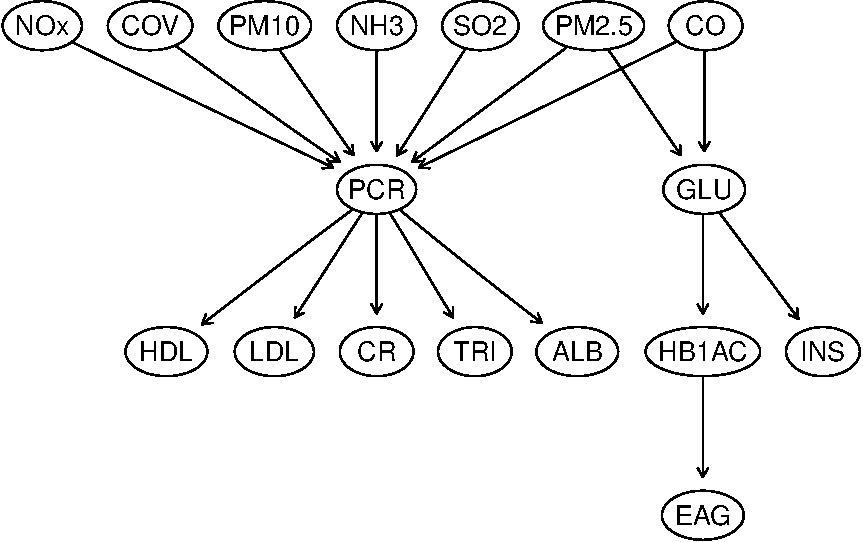
\includegraphics[keepaspectratio]{Reporte_files/figure-pdf/unnamed-chunk-21-1.pdf}}

\begin{Shaded}
\begin{Highlighting}[numbers=left,,]
\NormalTok{gbn3 }\OtherTok{=} \FunctionTok{bn.fit}\NormalTok{(dag3, }\AttributeTok{data =}\NormalTok{ data)}
\end{Highlighting}
\end{Shaded}

\begin{Shaded}
\begin{Highlighting}[numbers=left,,]
\NormalTok{score\_bic\_dag3 }\OtherTok{=} \FunctionTok{score}\NormalTok{(dag3, }\AttributeTok{data =}\NormalTok{ data, }\AttributeTok{type =} \StringTok{"bic{-}g"}\NormalTok{)}
\NormalTok{score\_bic\_dag3}
\end{Highlighting}
\end{Shaded}

\begin{verbatim}
[1] -97488.91
\end{verbatim}

\begin{Shaded}
\begin{Highlighting}[numbers=left,,]
\NormalTok{score\_aic\_dag3 }\OtherTok{=} \FunctionTok{score}\NormalTok{(dag3, }\AttributeTok{data =}\NormalTok{ data, }\AttributeTok{type =} \StringTok{"aic{-}g"}\NormalTok{)}
\NormalTok{score\_aic\_dag3}
\end{Highlighting}
\end{Shaded}

\begin{verbatim}
[1] -97361.97
\end{verbatim}

\begin{Shaded}
\begin{Highlighting}[numbers=left,,]
\CommentTok{\#tabla con los scores de las dag para que se vea bonita la comparacion}
\NormalTok{tabla\_scores }\OtherTok{\textless{}{-}} \FunctionTok{data.frame}\NormalTok{(}
  \AttributeTok{DAG =} \FunctionTok{c}\NormalTok{(}\StringTok{"DAG1"}\NormalTok{, }\StringTok{"DAG2"}\NormalTok{, }\StringTok{"DAG3"}\NormalTok{),}
  \AttributeTok{BIC =} \FunctionTok{c}\NormalTok{(score\_bic\_dag1, score\_bic\_dag2, score\_bic\_dag3),}
  \AttributeTok{AIC =} \FunctionTok{c}\NormalTok{(score\_aic\_dag1, score\_aic\_dag2, score\_aic\_dag3)}
\NormalTok{)}

\NormalTok{tabla\_scores}
\end{Highlighting}
\end{Shaded}

\begin{verbatim}
   DAG       BIC       AIC
1 DAG1 -97442.10 -97297.73
2 DAG2 -97471.69 -97344.75
3 DAG3 -97488.91 -97361.97
\end{verbatim}

Podemos observar que la DAG1 es la que presenta un menor error por lo
que va a ser la que usaremos en el resto del análisis. Una forma de
agregar una variable categórica, en este caso sexo, a la red gaussiana
sería recodificando la variable para volverla continua, o separar
nuestra base de datos en una de hombres y una de mujeres, trabajarlas
por separado, y ver cómo cambian las relaciones en ambas y comparar los
resultados de las inferencias condicionales que realicemos, este método
es el que realizaremos.

\begin{Shaded}
\begin{Highlighting}[numbers=left,,]
\NormalTok{data\_M }\OtherTok{=} \FunctionTok{read\_csv}\NormalTok{(}\StringTok{"../data/data\_M.csv"}\NormalTok{)}
\NormalTok{data\_F }\OtherTok{=} \FunctionTok{read\_csv}\NormalTok{(}\StringTok{"../data/data\_F.csv"}\NormalTok{)}
\FunctionTok{colnames}\NormalTok{(data\_M) }\OtherTok{\textless{}{-}} \FunctionTok{c}\NormalTok{(}\StringTok{"ALB"}\NormalTok{, }\StringTok{"HDL"}\NormalTok{, }\StringTok{"LDL"}\NormalTok{, }\StringTok{"CR"}\NormalTok{, }\StringTok{"GLU"}\NormalTok{, }\StringTok{"INS"}\NormalTok{, }\StringTok{"PCR"}\NormalTok{, }\StringTok{"TRI"}\NormalTok{, }\StringTok{"HB1AC"}\NormalTok{, }\StringTok{"EAG"}\NormalTok{, }\StringTok{"SO2"}\NormalTok{, }\StringTok{"CO"}\NormalTok{, }\StringTok{"NOx"}\NormalTok{, }\StringTok{"COV"}\NormalTok{, }\StringTok{"PM10"}\NormalTok{, }\StringTok{"PM2.5"}\NormalTok{, }\StringTok{"NH3"}\NormalTok{)}
\FunctionTok{colnames}\NormalTok{(data\_F) }\OtherTok{\textless{}{-}} \FunctionTok{c}\NormalTok{(}\StringTok{"ALB"}\NormalTok{, }\StringTok{"HDL"}\NormalTok{, }\StringTok{"LDL"}\NormalTok{, }\StringTok{"CR"}\NormalTok{, }\StringTok{"GLU"}\NormalTok{, }\StringTok{"INS"}\NormalTok{, }\StringTok{"PCR"}\NormalTok{, }\StringTok{"TRI"}\NormalTok{, }\StringTok{"HB1AC"}\NormalTok{, }\StringTok{"EAG"}\NormalTok{, }\StringTok{"SO2"}\NormalTok{, }\StringTok{"CO"}\NormalTok{, }\StringTok{"NOx"}\NormalTok{, }\StringTok{"COV"}\NormalTok{, }\StringTok{"PM10"}\NormalTok{, }\StringTok{"PM2.5"}\NormalTok{, }\StringTok{"NH3"}\NormalTok{)}
\end{Highlighting}
\end{Shaded}

\begin{Shaded}
\begin{Highlighting}[numbers=left,,]
\NormalTok{gbn\_masc }\OtherTok{=} \FunctionTok{bn.fit}\NormalTok{(dag1, }\AttributeTok{data =}\NormalTok{ data\_M)}
\NormalTok{gbn\_fem }\OtherTok{=} \FunctionTok{bn.fit}\NormalTok{(dag1, }\AttributeTok{data =}\NormalTok{ data\_F)}
\end{Highlighting}
\end{Shaded}

Queries: 1. ¿Cuál es la probabilidad de que una persona tenga los
triglicéridos saludables dado que están expuestas a altos niveles de
NOx?

\begin{Shaded}
\begin{Highlighting}[numbers=left,,]
\FunctionTok{cpquery}\NormalTok{(gbn1, }\AttributeTok{event =}\NormalTok{ (TRI }\SpecialCharTok{\textless{}} \DecValTok{200}\NormalTok{), }\AttributeTok{evidence =}\NormalTok{ (NOx }\SpecialCharTok{\textgreater{}} \FunctionTok{quantile}\NormalTok{(data}\SpecialCharTok{$}\NormalTok{NOx, }\FloatTok{0.8}\NormalTok{)), }\AttributeTok{n=}\DecValTok{10}\SpecialCharTok{\^{}}\DecValTok{6}\NormalTok{)}
\end{Highlighting}
\end{Shaded}

\begin{verbatim}
[1] 0.6536755
\end{verbatim}

¿Cuál sería la probabilidad sin condición?

\begin{Shaded}
\begin{Highlighting}[numbers=left,,]
\FunctionTok{cpquery}\NormalTok{(gbn1, }\AttributeTok{event =}\NormalTok{ (TRI }\SpecialCharTok{\textless{}} \DecValTok{200}\NormalTok{), }\AttributeTok{evidence =} \ConstantTok{TRUE}\NormalTok{, }\AttributeTok{n=}\DecValTok{10}\SpecialCharTok{\^{}}\DecValTok{6}\NormalTok{)}
\end{Highlighting}
\end{Shaded}

\begin{verbatim}
[1] 0.64335
\end{verbatim}

\begin{enumerate}
\def\labelenumi{\arabic{enumi}.}
\setcounter{enumi}{1}
\tightlist
\item
  ¿Cuál es la probabilidad de que los niveles de glucosa sean saludables
  en mujeres expuestas a altos niveles de COV y PM2.5?
\end{enumerate}

\begin{Shaded}
\begin{Highlighting}[numbers=left,,]
\FunctionTok{cpquery}\NormalTok{(gbn\_fem, }\AttributeTok{event =}\NormalTok{ (GLU }\SpecialCharTok{\textless{}} \DecValTok{100}\NormalTok{), }\AttributeTok{evidence =}\NormalTok{ (COV }\SpecialCharTok{\textgreater{}} \FunctionTok{quantile}\NormalTok{(data}\SpecialCharTok{$}\NormalTok{COV, }\FloatTok{0.8}\NormalTok{) }\SpecialCharTok{\&}\NormalTok{ PM2}\FloatTok{.5} \SpecialCharTok{\textgreater{}} \DecValTok{500}\NormalTok{), }\AttributeTok{n=}\DecValTok{10}\SpecialCharTok{\^{}}\DecValTok{6}\NormalTok{)}
\end{Highlighting}
\end{Shaded}

\begin{verbatim}
[1] 0.4508285
\end{verbatim}

¿Cuál sería la probabilidad sin condición?

\begin{Shaded}
\begin{Highlighting}[numbers=left,,]
\FunctionTok{cpquery}\NormalTok{(gbn\_fem, }\AttributeTok{event =}\NormalTok{ (GLU }\SpecialCharTok{\textless{}} \DecValTok{100}\NormalTok{), }\AttributeTok{evidence =} \ConstantTok{TRUE}\NormalTok{, }\AttributeTok{n=}\DecValTok{10}\SpecialCharTok{\^{}}\DecValTok{6}\NormalTok{)}
\end{Highlighting}
\end{Shaded}

\begin{verbatim}
[1] 0.461291
\end{verbatim}

\begin{enumerate}
\def\labelenumi{\arabic{enumi}.}
\setcounter{enumi}{2}
\tightlist
\item
  Cual es la probabilidad de que un hombre tenga un valor saludable de
  hemoglobina glucosilada dado que estan expuestos a altos niveles de CO
\end{enumerate}

\begin{Shaded}
\begin{Highlighting}[numbers=left,,]
\FunctionTok{cpquery}\NormalTok{(gbn1, }\AttributeTok{event =}\NormalTok{ (HB1AC }\SpecialCharTok{\textless{}} \DecValTok{6}\NormalTok{), }\AttributeTok{evidence =}\NormalTok{ (CO }\SpecialCharTok{\textgreater{}} \FunctionTok{quantile}\NormalTok{(data}\SpecialCharTok{$}\NormalTok{CO, }\FloatTok{0.8}\NormalTok{)), }\AttributeTok{n=}\DecValTok{10}\SpecialCharTok{\^{}}\DecValTok{6}\NormalTok{)}
\end{Highlighting}
\end{Shaded}

\begin{verbatim}
[1] 0.01352375
\end{verbatim}

¿Cuál sería la probabilidad sin condición?

\begin{Shaded}
\begin{Highlighting}[numbers=left,,]
\FunctionTok{cpquery}\NormalTok{(gbn1, }\AttributeTok{event =}\NormalTok{ (HB1AC }\SpecialCharTok{\textless{}} \DecValTok{6}\NormalTok{), }\AttributeTok{evidence =} \ConstantTok{TRUE}\NormalTok{, }\AttributeTok{n=}\DecValTok{10}\SpecialCharTok{\^{}}\DecValTok{6}\NormalTok{)}
\end{Highlighting}
\end{Shaded}

\begin{verbatim}
[1] 0.013185
\end{verbatim}

En general podemos observar que las probabilidades cambian muy poco, por
lo que podemos concluir que los contaminantes del aire no tienen impacto
en los biomarcadores de las personas.

Incluir modelos no paramétricos puede ayudar a mejorar el BIC y el AIC
si las relaciones entre los datos son no lineales o no gaussianas, ya
que los modelos no paramétricos permiten más flexibilidad en las
distribuciones condicionales, lo que permite capturar relaciones no
lineales.

Sin embargo, este acercamiento necesita una gran cantidad de datos para
evitar un sobreajuste y suele ser más difícil de interpretar.

\subsection{Conclusiones}\label{conclusiones}

Se construyeron tres modelos (DAGs) y, mediante los criterios AIC y BIC,
se seleccionó la estructura más adecuada. Sin embargo, los resultados de
las consultas condicionales mostraron que los cambios en la probabilidad
de presentar biomarcadores saludables ante altos niveles de
contaminantes fueron mínimos. Esto sugiere que, bajo los supuestos del
modelo, los contaminantes no presentan un impacto directo fuerte sobre
los biomarcadores analizados.

Una posible explicación es la limitación de las redes gaussianas, que
asumen relaciones lineales y distribuciones normales, lo cual puede no
reflejar la complejidad real de las interacciones entre contaminación y
salud. Para futuros trabajos, se recomienda el uso de modelos no
paramétricos o híbridos, así como bases de datos más amplias que
incluyan variables contextuales como hábitos de vida y condiciones
socioeconómicas. Aunque no se encontraron efectos significativos, la
metodología implementada constituye una base sólida para estudios
posteriores y puede convertirse en una herramienta útil para el diseño
de políticas públicas orientadas a la prevención de enfermedades
relacionadas con la contaminación.

\subsection{Referencias}\label{referencias}

https://www.jstatsoft.org/article/view/v035i03




\end{document}
